\subsection{Синтаксический анализатор} \label{sub113}

В~процессе компиляции синтаксический анализатор получает строку токенов от~лексического анализатора и~проверяет, может ли~эта строка имен токенов соответствовать грамматике исходного языка. Если программа написанна корректно, то синтаксический анализатор строит дерево разбора и~передает его следующей части компилятора для дальнейшей обработки. В противном случае синтаксический анализатор сообщает обо~всех выявленных ошибках и~продолжает работу с~оставшейся частью программы. 

Имеется три основных типа синтаксических анализаторов грамматик: 

\begin{itemize} 
	\item{\textit{Универсальные методы разбора}: например, алгоритмы Кока-Янгера-Касами (Cocke-Younger-Kasami) и~Эрли (Earley)~\cite{Earley1983}. Плюсами данного подхода является возможность работать с~любой грамматикой. Однако эти обобщённые методы слишком неэффективны для использования в~промышленных компиляторах и для реализации подобных алгоритмов требуются тьюринг-полные языки программирования.}
	\item{\textit{Восходящие методы разбора} (bottom-up): построение дерева разбора происходит снизу (от~листьев) вверх (к~корню). Поток токенов сканируется слева направо. Плюсом такого подхода является эффективный расход памяти (для реализации достаточно расширенного автомата с~магазинной памятью) и~близкая к~линейной оценка работы. }
	\item{\textit{Нисходящие методы разбора} (top-down): дерево разбора строится сверху (от~корня) вниз (к~листьям). Входной поток синтаксического анализатора, как и~в~восходящих методах, сканируется посимвольно слева направо. Такие методы используется для полностью ручной реализации, так как являются наиболее естественными для восприятия человеком.}
\end{itemize}

Пример разбора для выражения $-(\mathbf{id}+\mathbf{id})$ показан на~рис.~\ref{img:tree}

\begin{figure}[ht]
	\centering
	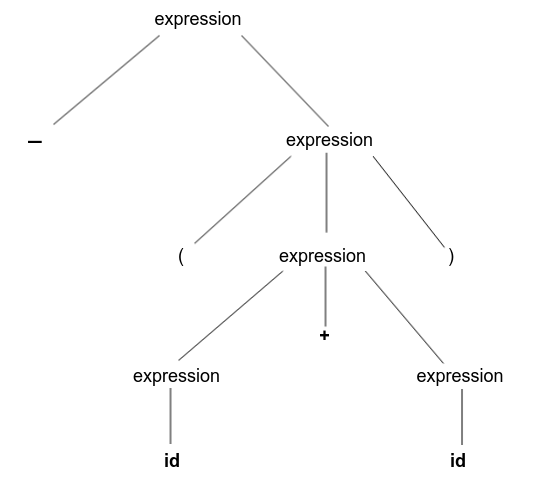
\includegraphics [scale=0.65]{tree}
	\caption{Дерево разбора для выражения $-(\mathbf{id}+\mathbf{id})$}
	\label{img:tree}
\end{figure}
